% Section 04 - Inverse Scattering Time Analysis

The Floquet-Fermi golden rule was proposed as an approach to analyze the transport properties of dressed quantum systems with impurities in Ref. \cite{wackerl20}.
However, this theory has not been applied for a dressed quantum Hall system in the previous studies. In this analysis, we use Floquet-Fermi golden rule to identify the effects induced by impurities on the magneto-transport properties.
With the help of $t-t'$ formalism \cite{wackerl20,grifoni98,sambe75,peskin93,althorpe97} and applying Floquet states derived in Eq.~(\ref{eq_12}), we can derive an  expression for $(l,l')$-th element of the inverse scattering time matrix for the $N$-th Landau level as
\begin{equation} \label{eq_13}
  \begin{aligned}
    \bigg(&\frac{1}{\tau(\varepsilon,k_x)}\bigg)^{ll'}_{N} \\
    & =
    \frac { \varrho^2}{eB}
    \delta(\varepsilon - \varepsilon_{N}) \\
    & \times
    \int_{-\infty}^{\infty} d k_1 \Bigg[
    J_l\qty(\frac{b\hbar}{eB}[{k}_x - k_1])
    J_{l'}\qty(\frac{b\hbar}{eB}[{k}_x - k_1]) \\
    & \times
    \qty|
    \int_{-\infty}^{\infty} dk_2 \;
    {\chi}_{N}\qty(\frac{\hbar}{eB}k_2)
    {\chi}_{N}\qty(\frac{\hbar}{eB} \qty[k_1 - {k}_x - k_2])|^2\Bigg],
  \end{aligned}
\end{equation}
where $\varrho = \eta_{imp} L_x [ { V_{imp}}/{eB}]^{1/2}$, $\varepsilon$ is a given energy value, $J_l(\cdot)$ are Bessel functions of the first kind with $l$-th integer order, and $\varepsilon_N$ is the energy of $N$-th Landau level.
Detailed derivation is given in Appendix \ref{appendix_c}.
We modeled the effect cause by impurities in the considering system by a single perturbation potential.
Since random impurities in a disordered metal is a better approximation for experimental results, we assumed that our perturbation potential is formed by a group of randomly distributed impurities.
Thus, the total scattering potential in 2DEG has been represented as a sum of uncorrelated single impurity potentials $\upsilon(\vb{r})$. Here $\eta_{imp}$ is the number of impurities in a unit area, $V_{imp} = \expval{|V_{{k'}_x,k_x}|^2}_{imp}$ with $V_{{k'}_x,k_x} = \mel**{k'_x}{\upsilon(x) }{k_x}$, and $\braket{x}{k_x} = e^{-ik_x x}$.
Moreover in this analysis, $\expval{\cdot}_{imp}$ represents the average over the impurity disorder.

Next we analyze the contribution of the inverse scattering time matrix elements on the transport properties of our system.
Since the disorder in the system can not alter the eigenenergy values of the undressed system \cite{wackerl20}, we can neglect the contribution of all off-diagonal elements in the inverse scattering time matrix. Then we consider only the central (${l=l'=0}$) diagonal element of the inverse scattering time matrix which has the largest contribution to the transport characteristics. Along with this assumption, we introduce a new parameter as the scattering-induced broadening of the $N$-th Landau level \cite{dini16,endo09}
\begin{equation} \label{eq_14}
 \Gamma^{00}_{N}(\varepsilon,k_x) = \hbar \qty(\frac{1}{\tau(\varepsilon,k_x)})^{00}_{N},
\end{equation}
and this leads to
\begin{equation} \label{eq_15}
 \begin{aligned}
   \Gamma^{00}_{N}& (\varepsilon,k_x) \\
   & =
   \frac { \varrho^2}{eB}
   \delta(\varepsilon - \varepsilon_{N}) \\
   & \times
   \int_{-\infty}^{\infty} d k_1 \Bigg[
   J_0^2\qty(\frac{b\hbar}{eB}[{k}_x - k_1])
   \\
   & \times
   \qty|
   \int_{-\infty}^{\infty} dk_2 \;
   {\chi}_{N}\qty(\frac{\hbar}{eB}k_2)
   {\chi}_{N}\qty(\frac{\hbar}{eB} \qty[k_1 - {k}_x - k_2])|^2\Bigg].
 \end{aligned}
\end{equation}

\begin{figure}[t]
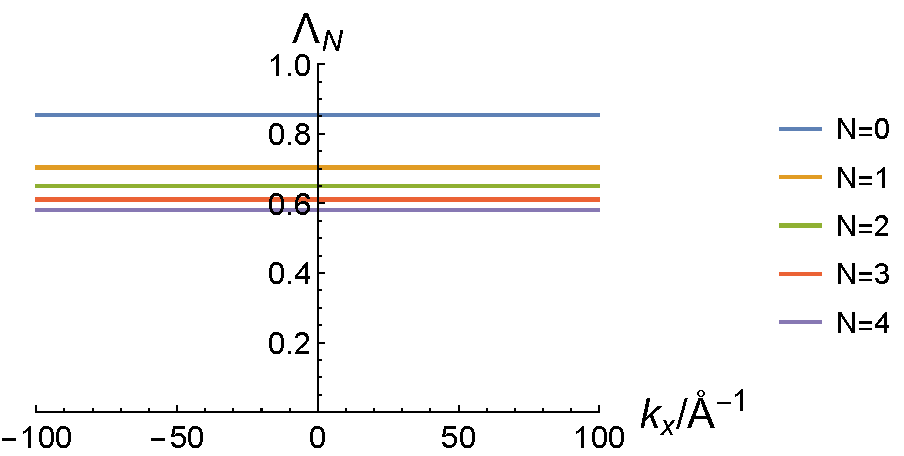
\includegraphics[scale=0.68]{figures/fig_3}
\caption{\label{fig_3} The dependence of normalized scattering-induced broadening $\Lambda_N$ for each Landau level ($N =0,1,2,3,4$) against $x$-directional momentum value $k_x$ in a GaAs-based quantum well under a nonoscillating magnetic field with $B = 1.2~\text{T}$, dressing field with frequency of $\omega =2\times10^{12}~\text{rad}\text{s}^{-1}$ and intensity $I =100~\text{W}/\text{cm}^{2}$.
In this calculation we have assumed that the natural  broadening of $0$-th Landau level $\Gamma_0$ is $0.24\;\text{me}V$.}
\end{figure}

\begin{figure}[b]
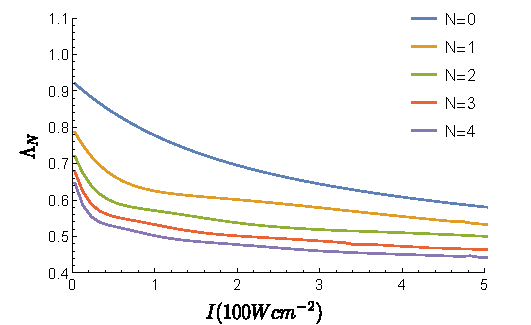
\includegraphics[scale=0.68]{figures/fig_4}
\caption{\label{fig_4} The dependence of normalized scattering-induced broadening $\Lambda_N$ for each Landau level ($N =0,1,2,3,4$) against dressing field intensity $I$, in a GaAs-based quantum well under a nonoscillating magnetic field with $B = 1.2~\text{T}$, dressing field with frequency of $\omega =2\times10^{12}~\text{rad}\text{s}^{-1}$. In this calculation we have assumed that the natural broadening of $0$-th Landau level $\Gamma_0$ is $0.24\;\text{me}V$.}
\end{figure}

In addition, for a scenario of scattering take place inside the same Landau level, we are able to present the delta distribution of the energy using the following interpretation \cite{dini16}
\begin{equation} \label{eq_16}
 \delta(\varepsilon - \varepsilon_{N}) \approx
 \frac{1}{\pi \Gamma^{00}_{N}(\varepsilon,k_x)}.
\end{equation}
Then we can write the central element of inverse scattering time matrix in more compact form
\begin{equation} \label{eq_17}
  \begin{aligned}
    \Gamma^{00}_{N}(\varepsilon,& k_x) =
    \varrho
    \bigg[
    \int_{-\infty}^{\infty} d {k}_1 \;
    J_0^2\qty(\lambda_1[{k}_x - {k}_1]) \\
    & \times
    \qty|
    \int_{-\infty}^{\infty} d{k}_2 \;
    \tilde{\chi}_{N}\qty(\lambda_2 k_2)
    \tilde{\chi}_{N}\qty(\lambda_2 \qty[{k}_1 - {k}_2 - {k}_x])|^2
    \bigg]^{-\frac{1}{2}},
  \end{aligned}
\end{equation}
where $ \lambda_1 \equiv \hbar b/eB$ and  $\lambda_2 \equiv \hbar \kappa/eB$.
To analyze the effect done by the dressing field on the scattering-induced broadening, we can introduce normalized $N$-th Landau level scattering-induced broadening as
\begin{equation} \label{eq_18}
    \Lambda_N(k_x) \equiv
    \frac{\Gamma^{00}_{N}(\varepsilon,k_x)}{\Gamma^{00}_{N=0}(\varepsilon,k_x)\big|_{E=0}},
\end{equation}
and this leads to
\begin{widetext}
\begin{equation} \label{eq_19}
    \Lambda_N (k_x) =
    \qty[
    \frac
    {\int_{-\infty}^{\infty} d {k}_1 \;
    J_0^2\qty(\lambda_1[{k}_x - {k}_1])
    \qty|
    \int_{-\infty}^{\infty} d{k}_2 \;
    \tilde{\chi}_{N}\qty(\lambda_2 k_2)
    \tilde{\chi}_{N}\qty(\lambda_2 \qty[{k}_1 - {k}_2 - {k}_x])|^2}
    {\int_{-\infty}^{\infty} d {k}_1 \;
    \qty|
    \int_{-\infty}^{\infty} d{k}_2 \;
    \tilde{\chi}_{0}\qty(\lambda_2 k_2)
    \tilde{\chi}_{0}\qty(\lambda_2 \qty[{k}_1 - {k}_2 - {k}_x])|^2}
    ]^{1/2}.
\end{equation}
\end{widetext}

Normalized energy band broadening against x-directional momentum component ${k_x}$ for different Landau levels ($N = 0,1,2,3,4$) has been calculated for GaAs-based quantum well and results are depicted in Fig.~(\ref{fig_3}) and Fig.~(\ref{fig_4}). To make a comparison, we have selected the experiment parameters to match with analysis done in Ref.~\cite{endo09}.
In their study, they have assumed that effective mass of the electron in GaAs-based quantum well system is $m_e \approx 0.07\tilde{m}_e$ where $\tilde{m}_e$ is mass of the electron \cite{endo09,winkler03,wackerl20}. In addition, they used the broadening of the natural(without a dressing field) $0$-th Landau level $\Gamma_0$ as $0.24\;\text{me}V$. Therefore, in our calculations, we assumed that the natural least Landau level broadening also has this value: $\Gamma^{00}_{N=0}|_{E=0} = 0.24 \;\text{meV}$.
Here we can identify that the normalized energy broadening value for each Landau level is independent of the x-directional momentum $k_x$ value and we are able to manipulate it by the dressing field. When the dressing field's intensity increase, the energy broadening gets reduced and this make adjustments in transport properties. In the next section, we are going to derive a analytical expression for the conductivity in dressed quantum Hall systems to analyze these adjustments.
